\documentclass[14pt, conference]{IEEEtran}
\ifCLASSINFOpdf
\else
\fi

\IEEEoverridecommandlockouts

\usepackage{listings}
\usepackage[table, svgnames]{xcolor}
\definecolor{codegreen}{rgb}{0,0.6,0}
\definecolor{codegray}{rgb}{0.5,0.5,0.5}
\definecolor{codepurple}{rgb}{0.58,0,0.82}
\definecolor{backcolour}{rgb}{0.5,1,0.5}
 
\lstdefinestyle{mystyle}{
    backgroundcolor=\color{backcolour},   
    commentstyle=\color{codegreen},
    keywordstyle=\color{magenta},
    numberstyle=\tiny\color{codegray},
    stringstyle=\color{codepurple},
    basicstyle=\footnotesize,
    breakatwhitespace=false,         
    breaklines=true,                 
    captionpos=b,                    
    keepspaces=true,                 
    numbers=none,                    
    numbersep=5pt,                  
    showspaces=false,                
    showstringspaces=false,
    showtabs=false,                  
    tabsize=2
}
 
\lstset{style=mystyle}


\usepackage{float}
\usepackage{longtable}
\usepackage{graphicx}
\usepackage{multirow}
%\usepackage{subcaption}
\usepackage{flushend}
\usepackage{hyperref}
\usepackage{tabularx} 
\usepackage{booktabs} % For formal tables
\usepackage{hhline}
\usepackage{array}

\colorlet{headercolour}{DarkSeaGreen}
\AtBeginEnvironment{tabular}{\rowcolors{1}{\ifnumequal{\rownum}{1}{headercolour}{white}}{}}%

\newcolumntype{L}[1]{>{\raggedright\let\newline\\\arraybackslash\hspace{0pt}}m{#1}}
\newcolumntype{C}[1]{>{\centering\let\newline\\\arraybackslash\hspace{0pt}}m{#1}}
\newcolumntype{R}[1]{>{\raggedleft\let\newline\\\arraybackslash\hspace{0pt}}m{#1}}
\bibliographystyle{IEEEtran}

\usepackage{cite}
\usepackage{amsmath,amssymb,amsfonts}
\usepackage{algorithmic}
\usepackage{graphicx}
\usepackage{textcomp}
\def\BibTeX{{\rm B\kern-.05em{\sc i\kern-.025em b}\kern-.08em
    T\kern-.1667em\lower.7ex\hbox{E}\kern-.125emX}}

\begin{document}

\title{Anomaly Detection Using Ensemble of Machine Learning Models}

\author{
\IEEEauthorblockN{Md. Khairul Islam\textsuperscript{1},
Prithula Hridi\textsuperscript{1}, Md. Shohrab Hossain\textsuperscript{1}, Husnu S. Narman\textsuperscript{2}}
\IEEEauthorblockA{\textsuperscript{1}Department of Computer Science and Engineering, Bangladesh University of Engineering and Technology, Bangladesh\\
    \textsuperscript{2}Weisberg Division of Computer Science, Marshall University, Huntington, WV, USA\\}
\IEEEauthorblockA{Email:  khairulislamtanim@gmail.com, prithula5117@gmail.com, mshohrabhossain@cse.buet.ac.bd,  narman@marshall.edu}
}

\maketitle

\begin{abstract}

Network intrusion detection systems help to find any security breaches inside the system. Anomaly detection system plays a significant role in recognizing intruders or suspicious activities inside the system, catching unseen and unknown attacks. Despite it has the weakness of having high false alarm rate, it can detect zero day attacks effectively which makes it more appropriate in scenarios where new attacks are common incidents. However benchmark anomaly detection datasets on modern traffic data are rare. In this paper, we have  worked on a data set\cite{moustafa2015unsw}~that reflects modern day network traffics. We have proposed  an ensemble based machine learning for anomaly detection from the network traffic. We have presented our results in terms of detection rate and accuracy. Our results outperforms the state of the art model proposed by Moustofa et al.~\cite{moustafa2018anomaly}.
\end{abstract}

\begin{IEEEkeywords}
anomaly, machine learning, network
\end{IEEEkeywords}
%------------------------ Into \input{introduction.tex}

\section{Introduction}

As web applications are being increasingly popular, internet has become a necessity in our day to day life. As a consequence, network systems are being targeted more by attacker with malicious intents. As stated in Verizon's Data Breach Investigation Report 2014, 63,437 security breaches carried out by hackers (Verizon's data breach investigation report, 2014 \footnote{http://www.verizonenterprise.com/DBIR/2014}). Also hacking tools are being more available.

To detect intruders in network system, there are generally two approaches : signature based and anomaly based. Signature based systems maintains database of previously known attacks and raise alarms in if when any match is found with the analyzed data. However they are vulnerable  to zero-day attacks.

Anomaly based detection (also known  as outlier detection, novelty detection, deviation detection, exception mining) is based on normal behaviour parameters and utilizes them to pinpoint any action that deviates significantly from normal behaviour. An anomaly in a network means deviation of traffic data from its normal pattern. So anomaly detection techniques has the advantage of detecting zero-day attacks. However in a complex and large network system it is not easy to define a set of valid requests or normal behavior. So anomaly detection faces the disadvantage of having high false positive rate error (events erroneously classified as attacks) .

Evaluating Network Intrusion Detection Systems (NIDS) using the existing benchmark data sets of KDD99 and NSLKDD does not reflect satisfactory results due to their lack of modern attack styles, traffic scenarios. To address these issues, the UNSW-NB15 data set was introduced by moustafa et al.~\cite{moustafa2015unsw}. This dataset represents a hybrid of real world and modern synthesized attack of network. It is a labeled dataset where supervised learning methods can be applied.

The state of the art work on this dataset is done in \cite{moustafa2018anomaly}, where they used a beta mixture model. Mixture models are probabilistic models for representing sub-populations within an overall population. After increasing weight (w) to 3, their model reaches upto 93.4\% accuracy, 92.7\% detection rate and 5.9\% false positive rate. Also in \cite{nawir2018multi}, the authors worked on multiclass classification of this dataset using AODE, an online learning algorithm.
However, to best of our knowledge, using recent machine learning and deep learning based techniques extensively on this dataset is yet to be explored. More over the the  false positive rate is quite high in~\cite{moustafa2018anomaly}. 

Our objective is to improve the detection  detection rate of  by using techniques, such as boosting or ensemble of multiple models that is being used frequently to make models more robust and general. 

In this paper, we have proposed an ensemble-based anomaly detection model trained and tested on  the unsw-nb15 dataset \cite{moustafa2015unsw}. This model outperforms the state of the art \cite{moustafa2018anomaly} in terms of detection rate (DR) and accuracy. Our model achieved 97.82\% DR , where the previous best is 92.70\%. Our achieved accuracy is 93.69\%, where previous best is 93.40\%. However, our model has higher false positive rate 15.11\%, compared to their 5.90\% , making the model prone to false alarms.


We hypertuned common machine learning and deep learning based models on the dataset. Then ensemble the best performing models using another neural network based model to give the final output. Our ensembled models are RandomForest, GradientBoosting, XGB, LightGBM, Neural Network(dense layer based).

The rest of the paper is organized as follows. In Section \ref{}, we have  propose our detection methodology. Details about the dataset and performance metrics are described in Section~\ref{sec:exp}. Results of our approach are presented in Section~\ref{sec:result}. Finally, Section \ref{sec:conclusion} has the concluding remarks.

We have discussed the experiments and their results in details in \ref{results}. Our comparisons with the current state of the art is given in \ref{comparison_table}.


Also being able to detect more attacks will make the model more vigorous against malicious traffics.


%-------------------------------------------------------------
%--- \input{motivation.tex}
%-------------------------------------------------------------
%\section{Background Study}
 There are different type of anomalies that can be mapped with different types of attacks~\cite{ahmed2016survey}. The main attacks are DoS, Probe, U2R and R2U attack.

The differnt types of anomalies are as follows:
\begin{itemize}
    \item \textbf{Point anomaly}:Rather than on the whole dataset, point anomaly occurs on a specific data instance.
    \item \textbf{Contextual anomaly}: When data instances are anomalous in a specific context, that can be called contextual anomaly. Like during season of festivities, credit card transactions are higher than regular. But it is not the same case for a non-festive season. High expenditure in a non-festive season can be pointed as a contextual anomaly. Occurrence of contextual anomalies depends on the availability of context attributes in the data. ~\cite{chandola2009anomaly}.
    \item \textbf{Collective anomaly}: When a collection of similar kind of data instances act anomalously with respect to the whole dataset, then it can be deemed as collective anomaly~\cite{ahmed2016survey}.
    
\end{itemize}

\begin{figure}[tb]
  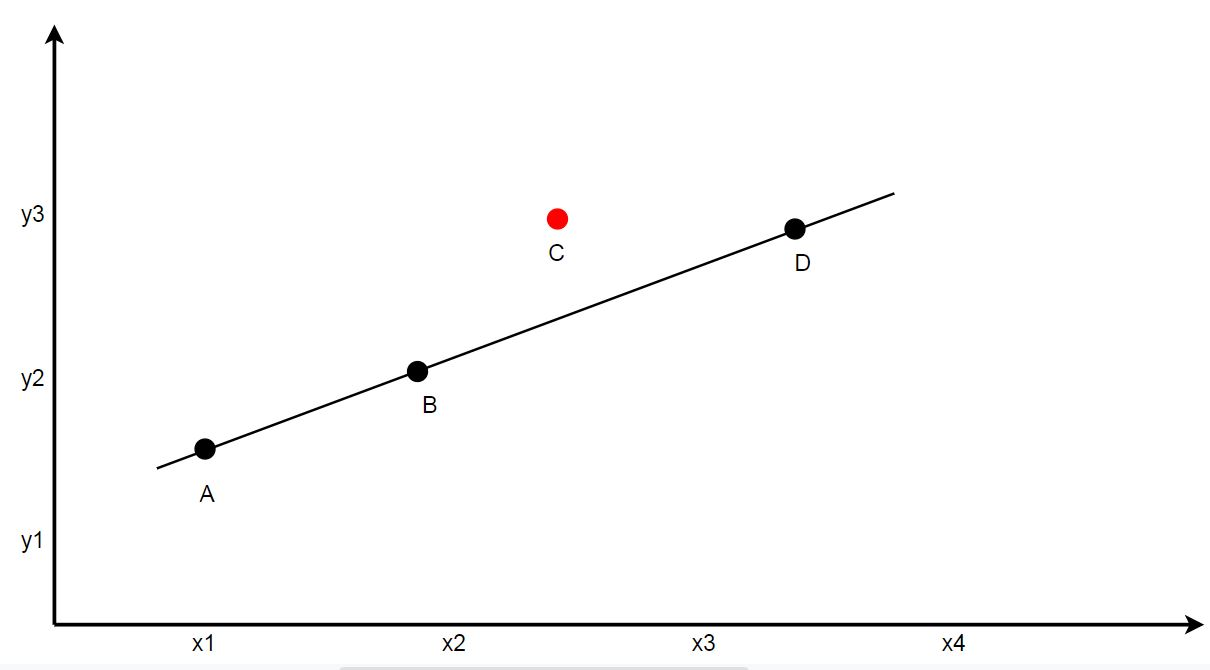
\includegraphics[width=\linewidth]{point.JPG}
  \caption{C is showing point anomaly.}
  \label{fig:point}
\end{figure}

\begin{figure}[bth]
  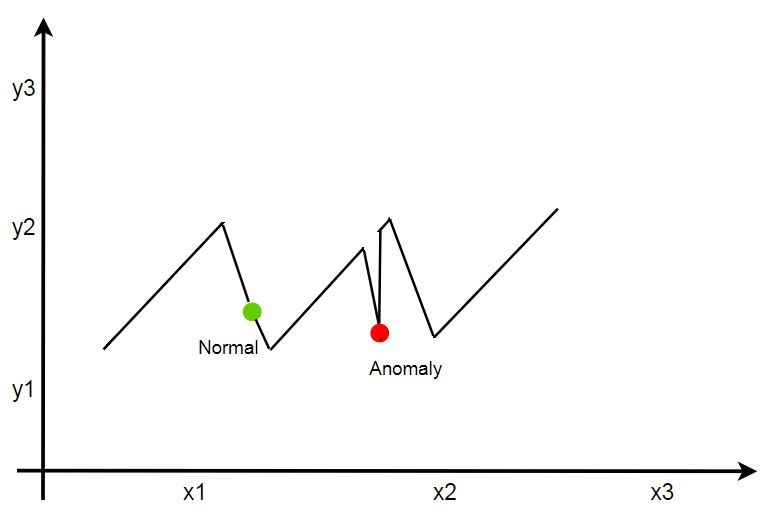
\includegraphics[width=\linewidth]{contextual.JPG}
  \caption{Contextual anomaly.}
  \label{fig:point}
\end{figure}

\begin{figure}[h]
  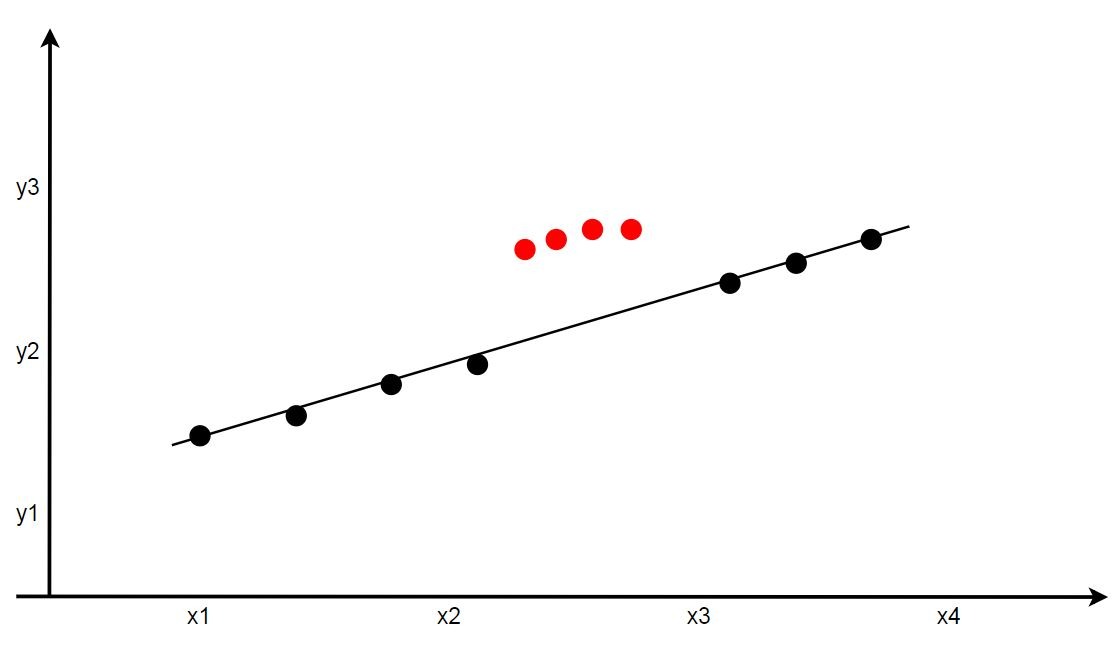
\includegraphics[width=\linewidth]{collective.JPG}
  \caption{4 red points are collectively showing anomaly.}
  \label{fig:point}
\end{figure}

There are different types of  attacks as follows:

\begin{itemize}
    \item \textbf{DoS attack}: DoS or Denial of Service represents the type of attack where the attacker makes a machine or resource unavailable to the legit users by blocking it intentionally through flooding. This attack keeps the memory resources of the server full so that legitimate user requests can not get through. Therefore, the user requests are denied.
    \item \textbf{Probe attack}: This type of attack is used to gather information about a targeted network or host and, more formally, for reconnaissance purposes ~\cite{ahmed2016survey}. This is used to know about the number \& type of machines connected in the network \& to know about installed softwares in the host machine. This is the step before an actual attack.
    \item \textbf{User to Root (U2R)}: When attacker wants to gain illegal access to an administrative account, U2R attack is used. Attacker can use social engineering approach or password sniffing \& being successful on those efforts, can access a normal user account. After gaining access in normal account \& exploiting vulnerabilities, attacker can gain the privilege of a super user.
    \item \textbf{Remote to User (R2U)}: It is launched when an attacker wants to gain local access as a user of a targeted machine to have the privilege of sending packets over its network (also known as R2L) ~\cite{ahmed2016survey}. Normally the attacker uses a trial and error method to guess the password. In some sophisticated attacks, attacker installs a sniffing tool to capture the password before going through the system.
\end{itemize}

Ahmed et al. ~\cite{ahmed2016survey} mapped the point anomaly with the U2R \& the R2U attacks. These type of attacks are condition specific and are hard to launch compared to other attacks. They mapped DoS attack to collective anomaly ~\cite{ahmed2014network} and Probe attack to contextual anomaly. DoS attack is specified by the collective attack of same nature. That is why it is mapped to collective anomaly as numerous connection requests are sent to deliver this attack. As probing is done on specific intention of gathering information, it is mapped with contextual anomaly.

\begin{figure}[b]
  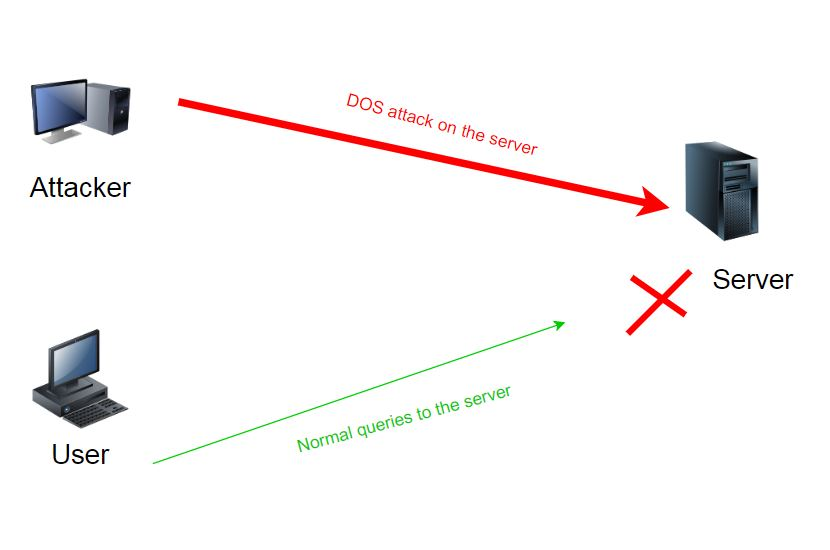
\includegraphics[width=\linewidth]{DOS2.JPG}
  \caption{DOS attack.}
  \label{fig:DOS}
\end{figure}



\section{Background Study}
 There are different type of anomalies that can be mapped with different types of attacks~\cite{ahmed2016survey}. The main attacks are DoS, Probe, U2R and R2U attack.

The different types of anomalies are as follows:
\begin{itemize}
    \item \textbf{Point anomaly}:Rather than on the whole dataset, point anomaly occurs on a specific data instance.
    \item \textbf{Contextual anomaly}: When data instances are anomalous in a specific context, that can be called contextual anomaly. Like during season of festivities, credit card transactions are higher than regular. But it is not the same case for a non-festive season. High expenditure in a non-festive season can be pointed as a contextual anomaly. Occurrence of contextual anomalies depends on the availability of context attributes in the data. ~\cite{chandola2009anomaly}.
    \item \textbf{Collective anomaly}: When a collection of similar kind of data instances act anomalously with respect to the whole dataset, then it can be deemed as collective anomaly~\cite{ahmed2016survey}.
    
\end{itemize}

\begin{figure}[tb]
  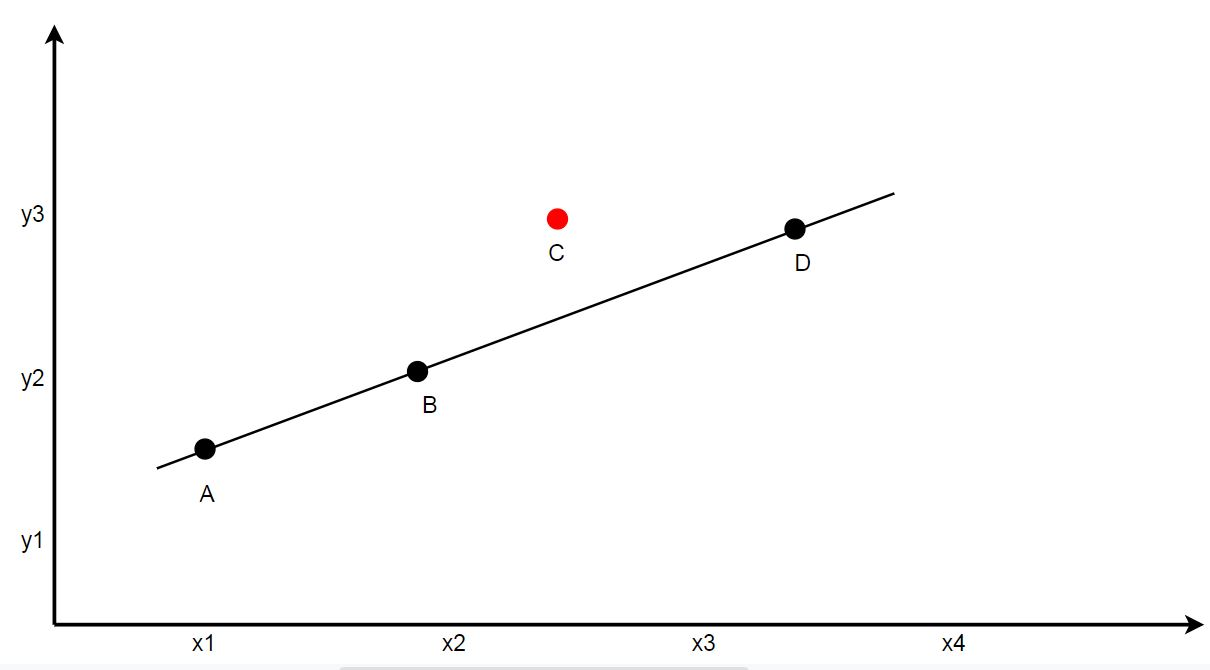
\includegraphics[width=\linewidth]{point.JPG}
  \caption{C is showing point anomaly.}
  \label{fig:point}
\end{figure}

\begin{figure}[bth]
  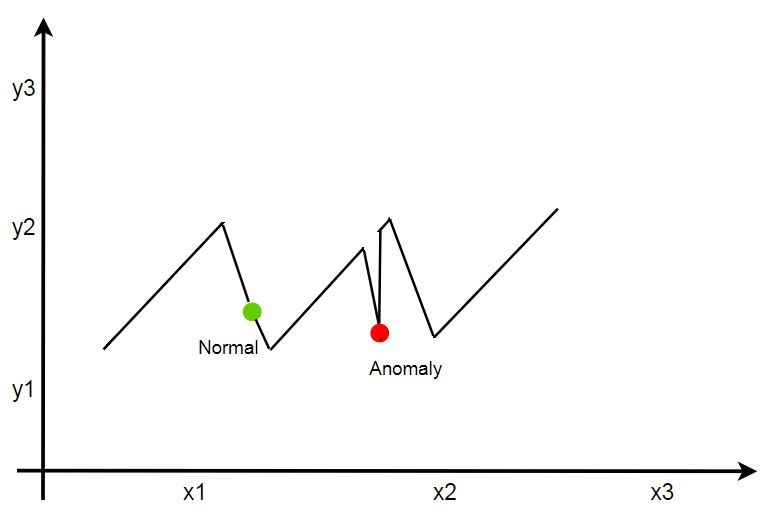
\includegraphics[width=\linewidth]{contextual.JPG}
  \caption{Contextual anomaly.}
  \label{fig:point}
\end{figure}

\begin{figure}[h]
  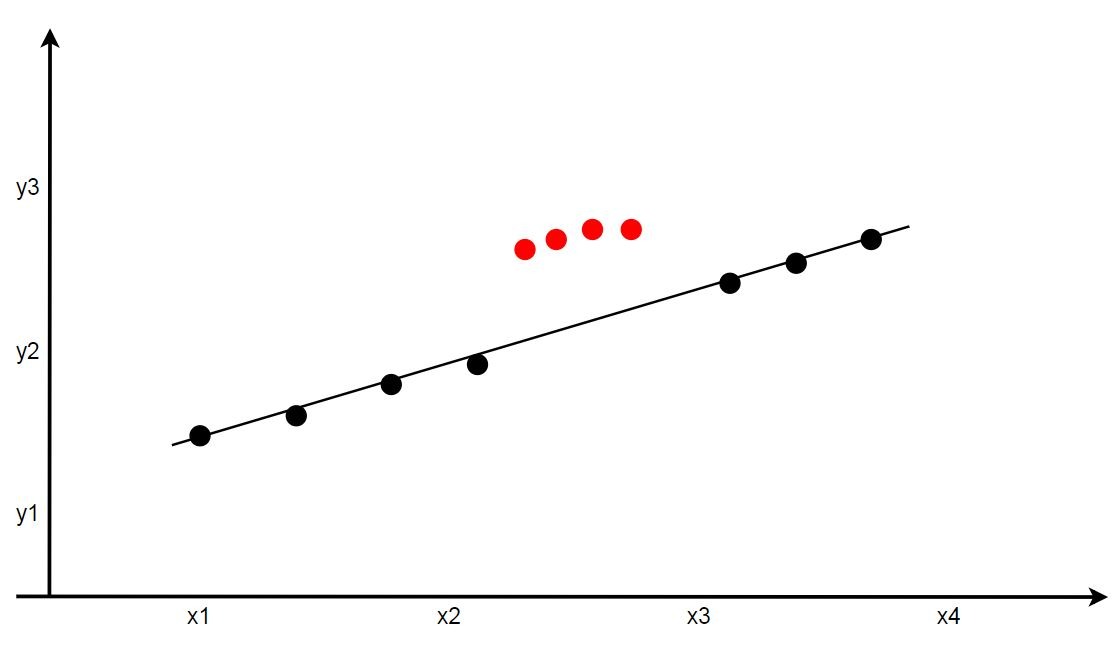
\includegraphics[width=\linewidth]{collective.JPG}
  \caption{4 red points are collectively showing anomaly.}
  \label{fig:point}
\end{figure}

There are different types of  attacks as follows:

\begin{itemize}
    \item \textbf{DoS attack}: DoS or Denial of Service represents the type of attack where the attacker makes a machine or resource unavailable to the legit users by blocking it intentionally through flooding. This attack keeps the memory resources of the server full so that legitimate user requests can not get through. Therefore, the user requests are denied.
    \item \textbf{Probe attack}: This type of attack is used to gather information about a targeted network or host and, more formally, for reconnaissance purposes ~\cite{ahmed2016survey}. This is used to know about the number \& type of machines connected in the network \& to know about installed software in the host machine. This is the step before an actual attack.
    \item \textbf{User to Root (U2R)}: When attacker wants to gain illegal access to an administrative account, U2R attack is used. Attacker can use social engineering approach or password sniffing \& being successful on those efforts, can access a normal user account. After gaining access in normal account \& exploiting vulnerabilities, attacker can gain the privilege of a super user.
    \item \textbf{Remote to User (R2U)}: It is launched when an attacker wants to gain local access as a user of a targeted machine to have the privilege of sending packets over its network (also known as R2L) ~\cite{ahmed2016survey}. Normally the attacker uses a trial and error method to guess the password. In some sophisticated attacks, attacker installs a sniffing tool to capture the password before going through the system.
\end{itemize}

Ahmed et al. ~\cite{ahmed2016survey} mapped the point anomaly with the U2R \& the R2U attacks. These type of attacks are condition specific and are hard to launch compared to other attacks. They mapped DoS attack to collective anomaly ~\cite{ahmed2014network} and Probe attack to contextual anomaly. DoS attack is specified by the collective attack of same nature. That is why it is mapped to collective anomaly as numerous connection requests are sent to deliver this attack. As probing is done on specific intention of gathering information, it is mapped with contextual anomaly.

\begin{figure}[b]
  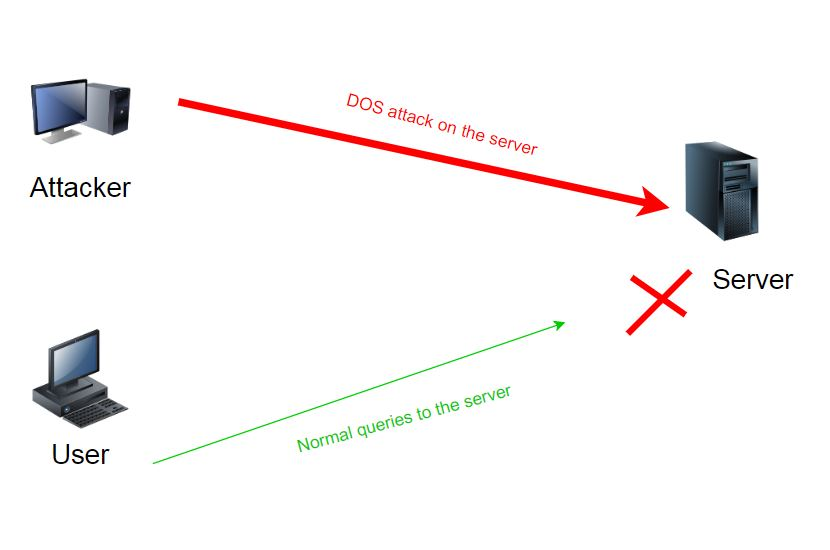
\includegraphics[width=\linewidth]{DOS2.JPG}
  \caption{DOS attack.}
  \label{fig:DOS}
\end{figure}

%---------------------------------------
%\input{related_works.tex}
\section{Literature Review}
Anomaly detection techniques can be classified into  four major  categories~\cite{ahmed2014network} as follows:

\begin{itemize}
\item Classification based techniques
\item Statistical based techniques
\item Clustering based techniques
\item Information Theory based techniques
\end{itemize}

Classification based techniques rely on experts' extensive knowledge of the characteristics of network attack.
SVM, Rule-based, Neural Network based techniques are under this type. This type of techniques rely on the normal traffic activity profile that builds the knowledge base and consider activities that deviates from baseline profile as anomalous. The advantage of this type of technique is they have ability to detect novel attacks provided that they show an ample deviation. The common disadvantage is that the normal profiles not included in the knowledge base will create false alarms.

Eskin et al. ~\cite{eskin2002geometric} used the concept of the unsupervised SVM to detect anomalous events. The algorithm finds hyper planes which separate the data instances from their origins with the maximal margin and then an optimization problem is solved to determine the best hyper plane. Hu et al. ~\cite{hu2003robust} presented an anomaly detection method which ignores noisy data is developed using the Robust SVM (RSVM).\\

Practically, training data often contain noise. This invalidates the main assumption of the SVM that all the sample data for training are independently and identically distributed. As a result, the standard SVM results in a highly non-linear decision boundary which leads to poor generalization.
In this scenario, the RSVM incorporates the averaging technique in the form of a class centre to make the decision surface smoother and automatically control regularization. In addition, the number/ quantity of support vectors in the RSVM is significantly less than the standard SVM which results in a reduced run time

One of the recent works on NSL-KDD (2009) dataset is done by Yin et al. ~\cite{yin2017deep}.They used a deep learning using recurrent neural networks (RNN). They found that RNN based approach gives superior performance to other classical machine learning approaches.
They have shown that their model can attain 81.29\% accuracy.

Another recent research done by Zhu et al. ~\cite{zhu2018deep} also uses a deep learning based approach. They used the attention-base Multi-Flow LSTM. LSTM is used to find the hidden temporal correlation between traffic flows. Here previous traffic flows are used as auxiliary features. They used CICIDS2017 dataset which included up-to-date common attacks.

One of the major problems in the field of anomaly detection based intrusion detection is want of benchmark dataset. Moustafa and Slay discussed about the new UNSW-NB15 dataset in ~\cite{moustafa2015unsw}. Their focus was on the point that the other datasets were not enough to tackle the modern low footprint attacks. They have also done a statistical analysis of the UNSW-NB15 dataset and compared it with the KDD99 dataset in ~\cite{moustafa2016evaluation}. Here they addressed three issues, lack of modern low footprint attack, lack of modern traffic scenarios \& the difference in the distribution of training and testing sets. According to them these are the major issues with the benchmark KDD99 \& NSLKDD datasets.

In ~\cite{moustafa2018anomaly}, Moustafa, Nour, et al. developed an anomaly detection system using beta mixture model. They evaluated their method on UNSW-NB15 dataset. They mentioned three components of anomaly detection system. They are data source, data pre-processing and decision-making method. Accuracy increased from 84.2 to 93.4 while the w value increased from 1.5 to 3. They have also shown that their BMM-ADS technique comes with higher detection rate (DR) \& lower false positive rate (FPR) than recent 3 methods evaluated on this dataset, Multivariate Correlation Analysis ~\cite{tan2014system} (DR 88.3 \& FPR 11.6), Artificial Immune System ~\cite{saurabh2016efficient} (DR 83.5 \& FPR 15.7), filter-based Feature Selection ~\cite{ambusaidi2016building} (DR 90.4 \& FPR 8.5). They shown their algorithm has the detection rate \& false positive rate of 92.7 \& 5.9~\cite{moustafa2018anomaly} respectively.

In ~\cite{nawir2018multi}, Nawir et. al. gave an algorithm Online Average One Dependence Estimator (AODE) for multi-classification of UNSW-NB15 dataset that is high in accuracy with a low false alarm rate (FAR). This was built to overcome some issues like the nature of data (complex data which can be represented into more than two classes), dynamical data in a network system, and frequent update (for streaming data that need a
fast processing).

Moustafa, Nour et. al. have done some other works on the UNSW-NB15 dataset ~\cite{moustafa2018ensemble, moustafa2018generalized, moustafa2018network}.

\subsection{Current limitations and our contributions}
When studying current works we found that
\begin{enumerate}
    \item Machine learning and deep learning techniques haven't yet been extensively applied to this dataset.
    \item Ensemble technique, which mixes results from multiple models to make the final model more robust and general, is yet to apply on this dataset.
    \item Results on this dataset might be improved using the previous techniques. Enabling the model to detect more anomalies.
\end{enumerate}

So our contribution is this work is :
\begin{enumerate}
    \item Implementing machine learning and deep learning models with this dataset
    \item Ensemble the best performing models
    \item Comparison of latest machine learning techniques with previous statistic based technique at detecting anomalies
\end{enumerate}




%-------------------------------------------------------------
\input{methodology.tex}

\section{Proposed Approach}
\subsection{Dataset Description}
UNSW-NB15 dataset is represented as a hybrid of the real normal and modern synthesized attack of
network data. Since, the dataset is labelled, we have implemented ML algorithms for network anomaly
detection in supervised learning. For our work, the UNSW-NB15 dataset contains in total 257,673 data instances with 44 features. The total classes of this dataset are 10 classes: one
is for a normal network data and nine classes of anomalous network data (attacks
classes). The attacks involved were backdoor, analysis, fuzzers, shellcode, reconnaissance, exploits, DoS, worms , and generic. 
\begin{table}[ht]
% this increases the fontsize used in table
\normalsize

\centering
\caption{UNSW-NB15 dataset description}
\label{unsw_nb15_des}
% increases cell padding
\renewcommand{\arraystretch}{1.2}

\begin{tabular}{|C{3cm}|C{1.6cm}|C{1.6cm}|}
\hline
\textbf{Attack type} & \textbf{Train} & \textbf{Test} \\ \hline
Normal & 37000 & 56000  \\ \hline
Generic  &         18871 & 40000 \\ \hline
Exploits  &        11132 & 33393 \\ \hline
Fuzzers    &        6062 & 18184 \\ \hline
DoS         &       4089 & 12264 \\ \hline
Reconnaissance &    3496 &  10491 \\ \hline
Analysis    &        677 &  2000 \\ \hline
Backdoor     &       583 & 1746 \\ \hline
Shellcode     &      378 & 1133 \\ \hline
Worms         &       44 &  130 \\ \hline
\textbf{Total} & \textbf{82322}  & \textbf{175341} \\ \hline
\end{tabular}
\end{table}


\subsection{Pre-processing}
\subsubsection{Dropping unnecessary columns}
We dropped id columns from both train and test dataset as those can't be learned as features. Also source and destination IP address and port no was excluded from feature set.

\subsubsection{Numericalization}
As machine learning requires input data to be in numeric format, we converted each categorical column into numeric by creating binary columns for each of their attributes. However test set had 6 nominal values which never appeared in train dataset. They are PAR, ECO, URN, NO in state column and icmp, rtp in protocol column. As they were absent in train data, model had no way of learning from them. So we have dropped the binary columns for these labels. In final , we had 188 features in our train data set.

\subsubsection{Scaling}
We applied standard scaling using StandardScaler from sklearn's preprocessing library. This scaler calculates the mean and standard deviation of training  samples and converts them using the following equation: 
\begin{equation}
    x = \frac{x-mean}{standard\:deviation}
\end{equation}

\subsection{Evaluation metrics}
There are 4 important terms need to be discussed before going into the next phase:
\begin{itemize}
    \item \textbf{True Positives (TP)} : The cases in which we predicted YES and the actual output was also YES.
    \item \textbf{True Negatives (TN} : The cases in which we predicted NO and the actual output was NO.
    \item \textbf{False Positives (FP)} : The cases in which we predicted YES and the actual output was NO.
    \item \textbf{False Negatives (FN)} : The cases in which we predicted NO and the actual output was YES.
\end{itemize}

\subsubsection{Accuracy}
It is the ratio of number of correct predictions to the total number of input samples
\begin{equation}
    Accuracy = \frac{TP+TN}{TP+TN+FP+FN}
\end{equation}

\subsubsection{Precision}
It is the number of correct positive results divided by the number of positive results predicted by the classifier.
\begin{equation}
    precision = \frac{TP}{TP+FP}
\end{equation}

\subsubsection{Recall or DR(Detection Rate)}
It is the number of correct positive results divided by the number of all relevant samples (all samples that should have been identified as positive)
\begin{equation}
    recall = \frac{TP}{TP+FN}
\end{equation}

\subsubsection{FPR}
The false positive rate (FPR) is the proportion of incorrectly identified observations, that is 
\begin{equation}
    FPR = \frac{FP}{FP+TN}
\end{equation}

\subsubsection{F1-score}
F1-score is the harmonic Mean between precision and recall.
\begin{equation}
    f1-score = 2 * \frac{1}{\frac{1}{precision}+ \frac{1}{recall}}
\end{equation}


%\subsubsection{AUC}


%---------------------------- Results  ----------------
%\input{unsw_nb15.tex}
\section{Results }\label{results}
In this section we describe experimentation methods and results of various machine learning based models on unsw-nb15 dataset. In each part we have described the hypertuning part of a model and the best possible results from it. The best results are marked using * in each table.\\

\subsection{RandomForestClassifier}
We used RandomForestClassifier from sklearn.ensemble . Table \ref{rf_table} contains the hyper-tuning results. Base parameters of the classifier are given below.

\begin{table}[H]
% this increases the fontsize used in table
\normalsize

\centering
\caption{RandomForest baseline parameters}
\label{rf_base_parameters}
% increases cell padding
\renewcommand{\arraystretch}{1.2}

\begin{tabular}{|C{2.6cm}|C{1cm}|C{2.7cm}|C{1cm}|}
\hline
\textbf{parameter} & \textbf{value} & \textbf{parameter} & \textbf{value} \\ \hline
criterion & ’gini’ &  min\_samples\_split  & 2   \\ \hline
min\_samples\_leaf & 1 & class\_weight & None  \\ \hline
max\_features & ’auto’& max\_leaf\_nodes & None  \\ \hline
%min\_impurity\_decrease & 0.0 & min\_impurity\_split & None  \\ \hline
bootstrap & True & oob\_score & False  \\ \hline
warm\_start & False & random\_state & 0  \\ \hline
%min\_weight\_fraction\_leaf & 0.0 & &  \\ \hline
\end{tabular}
\end{table}

% \begin{lstlisting}[language=Python]

% RandomForestClassifier(n_estimators=’warn’, criterion=’gini’, max_depth=None, min_samples_split=2, min_samples_leaf=1, min_weight_fraction_leaf=0.0, max_features=’auto’, max_leaf_nodes=None, min_impurity_decrease=0.0, min_impurity_split=None, bootstrap=True, oob_score=False, n_jobs=None, random_state=None, verbose=0, warm_start=False, class_weight=None)

% \end{lstlisting}
We set prediction threshold at 0.4 for this model.From table \ref{rf_table} we can see that changing max depth didn't have much effect on the model performance except reducing it a bit. However the more we increased the number of estimators after 100 the less the results become.Possibly because model overfits on train data. Also decreasing less than 100 has negative effect on the performance. So the best model was achieved with 100 estimators and max depth at 50.

\begin{table}[H]
% this increases the fontsize used in table
\normalsize

\centering
\caption{RandomForest classifier results}
\label{rf_table}
% increases cell padding
\renewcommand{\arraystretch}{1.2}

\begin{tabular}{|C{2cm}|C{1.2cm}|C{1.6cm}|C{1.6cm}|}
\hline
\textbf{n-estimators} & \textbf{depth} & \textbf{accuracy} & \textbf{f1-score} \\ \hline
50 & 50 & 93.24 & 95.22 \\ \hline
50 & 150 & 93.33 & 95.27 \\ \hline
100 & 50 & 93.39* & 95.31* \\ \hline
100 & 150 & 93.33 & 95.27 \\ \hline
200 & 50 & 93.36 & 95.30 \\ \hline
200 & 150 & 93.34 & 95.29\\ \hline
500 & 50 & 93.03 & 95.31 \\ \hline
500 & 150 & 93.01 & 95.29 \\ \hline
\multicolumn{4}{l}{$*$ best parameters}
\end{tabular}
\end{table}

\subsection{GradientBoostingClassifier}
We used GradientBoostingClassifier from sklearn.ensemble. It builds an additive model in a forward stage-wise fashion; it allows for the optimization of arbitrary differentiable loss functions. As this is binary classification, in each stage a single regression tree is fit on the negative gradient of the binomial deviance loss function.The base parameters for this model are given in table \ref{gtb_base_parameters}.
\begin{table}[H]
% this increases the fontsize used in table
\normalsize

\centering
\caption{GradientBoostingClassifier baseline parameters}
\label{gtb_base_parameters}
% increases cell padding
\renewcommand{\arraystretch}{1.2}

\begin{tabular}{|C{2.7cm}|C{1cm}|C{2.6cm}|C{1cm}|}
\hline
\textbf{parameter} & \textbf{value} & \textbf{parameter} & \textbf{value} \\ \hline
learning\_rate & 0.1 & presort & ’auto’ \\ \hline
n\_estimators & 100 &  subsample & 1.0 \\ \hline
max\_depth & 3 &  tol & 0.0001 \\ \hline
random\_state & 0 & max\_features & None \\ \hline
\end{tabular}
\end{table}

% \begin{lstlisting}[language=Python]

% GradientBoostingClassifier(loss=’deviance’, learning_rate=0.1, n_estimators=100, subsample=1.0, criterion=’friedman_mse’, min_samples_split=2, min_samples_leaf=1, min_weight_fraction_leaf=0.0, max_depth=3, min_impurity_decrease=0.0, min_impurity_split=None, init=None, random_state=None, max_features=None, verbose=0, max_leaf_nodes=None, warm_start=False, presort=’auto’, validation_fraction=0.1, n_iter_no_change=None, tol=0.0001)
% \end{lstlisting}

We varied n\_estimators and learning rate for this model. Each estimator has regression trees with max depth 3. We set prediction threshold at 0.5 for this model. From table \ref{gtb_table} we see, the more we increased the number of estimators, the more performance increased. the more general the model became, hence the increase of performance. We didn't increase it further to prevent overfitting. Also decreasing learning rate than 0.1 had negative impact on performance, because the model was learning too slow to converge.
\begin{table}[H]
\normalsize

\centering
\caption{GradientBoosting Classifier results}
\label{gtb_table}
\renewcommand{\arraystretch}{1.2}
\begin{tabular}{|C{2cm}|C{2cm}|C{1.5cm}|C{1.5cm}|}
\hline
\textbf{n-estimators} & \textbf{learning rate} & \textbf{accuracy} & \textbf{f1-score} \\ \hline
100 & 0.01 & 85.42 & 88.74 \\ \hline
100 & 0.05 & 89.82 & 92.31 \\ \hline
100 & 0.1 & 92.09 & 94.12 \\ \hline
200 & 0.01 & 85.53 & 88.8 \\ \hline
200 & 0.05 & 92.42 & 94.48 \\ \hline
200 & 0.1 & 92.30 & 94.36 \\ \hline
500 & 0.01 & 91.26 & 93.44 \\ \hline
500 & 0.05 & 92.40 & 94.49 \\ \hline
500 & 0.1 & 92.61* & 94.67* \\ \hline
\multicolumn{4}{l}{$*$ best parameters}
\end{tabular}
\end{table}

\subsection{LightGBM}
LightGBM is a gradient boosting framework from Microsoft that uses tree based learning algorithms. The baseline parameters are given in table \ref{lgb_table}.

\begin{table}[H]
% this increases the fontsize used in table
\normalsize

\centering
\caption{LightGBM baseline parameters}
\label{lgb_base_parameters}
% increases cell padding
\renewcommand{\arraystretch}{1.2}

\begin{tabular}{|C{3.1cm}|C{.7cm}|C{2.6cm}|C{0.8cm}|}
\hline
\textbf{parameter} & \textbf{value} & \textbf{parameter} & \textbf{value} \\ \hline
bagging\_frequency & 5 & base\_score & 0.9 \\ \hline
early\_stopping\_round & 100 & num\_boost\_round & 2000 \\ \hline
boost & gbdt & max\_bin & 255\\ \hline
objective & binary & seed & 0 \\ \hline
num\_leaves & 31 & & \\ \hline
\end{tabular}
\end{table}

We varied 4 parameters of this model: learning rate, max-depth, bagging fraction, feature fraction. We set prediction threshold at 0.4 for this model. From table \ref{lgb_table} we can see, decreasing learning rate had a decrease in performance too. We found setting constraint on depth giving better results. Among them best results came at depth 10. Also adding fraction less than 1.0 improved classifier performance, this fraction means what fraction of the dataset and features would be used for training in the next iteration. 

\begin{table}[H]
\normalsize

\centering
\caption{LightGBM results}
\label{lgb_table}
\renewcommand{\arraystretch}{1.2}
\begin{tabular}{|C{1.4cm}|C{1.2cm}|C{1.6cm}|C{1.2cm}|C{1.2cm}|}
\hline
\textbf{learning rate} & \textbf{max depth} & \textbf{bagging and feature fraction} & \textbf{accuracy} & \textbf{f1-score} \\ \hline
0.1 & 10 & 0.5 & 92.69 & 94.71 \\ \hline
0.1 & 10 & 1 & 92.75* & 94.78* \\ \hline
0.1 & 15 & 0.5 & 92.63 & 94.69 \\ \hline
0.1 & 15 & 1 & 92.59 & 94.67 \\ \hline
0.01 & 10 & 0.5 & 92.75 & 94.69 \\ \hline
0.01 & 10 & 1 & 92.55 & 94.59 \\ \hline
0.01 & 15 & 0.5 & 92.84 & 94.76 \\ \hline
0.01 & 15 & 1 & 92.59 & 94.62 \\ \hline
\multicolumn{5}{l}{$*$ best parameters}
\end{tabular}
\end{table}

\subsection{XGBClassifier}
XGBoost is an optimized distributed gradient boosting library designed to be highly efficient, flexible and portable. It implements machine learning algorithms under the Gradient Boosting framework. In this approach we worked on the XGBClassifier from XGBoost.\\

We replaced the base score with 0.9, as it showed a bit improvement on the score. Then we varied n-estimators and learning rate. From table \ref{xgb_table} we can see, performance decreases randomly with the increase of number of estimators. However for learning rate it increased when going from 0.1 to 0.5. However increasing learning rate too much can make the model fail to converge. So for best result we kept the model at 100 n-estimators, 0.5 learning rate and 0.9 base-score. Prediction threshold was set to 0.2 for this model.
\begin{table}[H]
\normalsize
\centering
\caption{XGB Classifier results}
\label{xgb_table}

\renewcommand{\arraystretch}{1.2}
\begin{tabular}{|C{2cm}|C{2cm}|C{1.5cm}|C{1.5cm}|}
\hline
\textbf{n-estimators} & \textbf{learning rate} & \textbf{accuracy} & \textbf{f1-score} \\ \hline
100 & 0.1 & 91.45 & 93.71 \\ \hline
100 & 0.5 & 92.13* & 94.34* \\ \hline
500 & 0.1 & 91.94 & 94.23 \\ \hline
500 & 0.5 & 90.42 & 93.3 \\ \hline
1000 & 0.1 & 90.98 & 93.64 \\ \hline
1000 & 0.5 & 90.42 & 93.3 \\ \hline
\multicolumn{4}{l}{$*$ best parameters}
\end{tabular}
\end{table}

\subsection{Artificial Neural Network}
An ANN is based on a collection of connected units or nodes called artificial neurons, which loosely model the neurons in a biological brain. Each connection, like the synapses in a biological brain, can transmit a signal from one artificial neuron to another. An artificial neuron that receives a signal can process it and then signal additional artificial neurons connected to it.\\
Here in this experiment we used Keras \footnote{https://keras.io/}, a python deep learning library developed by Google. It is capable of running on top of TensorFlow, CNTK, or Theano.\\

We tried different combination of layers,units of dense and dropout layer.Dense layer is a densely connected neural network layer, which connects every input to every cell unit. Dropout layer randomly sets a fraction of input units to 0, reducing overfit. However if we drop too much that will cause the model to underfit. \\

Our number of epochs were 10 and we took the best model based on validation accuracy. From our results in \ref{nn_table}, we can see increasing input layer size increases model performance, possibly because it helps to learn more from the input data. However using more layers cause the model to overfit, doing well on train data, but reducing performance on test data. Also adding dropout layer didn't solve the issue. So the best model was a NN with 512 dense input units, then 32 dense input units, following the final output unit. All dense layers except the last one used activation method 'relu'.\\
\begin{table}[H]
\normalsize

\centering
\caption{ANN results}
\label{nn_table}
\renewcommand{\arraystretch}{1.2}
\begin{tabular}{|C{5.6cm}|C{1cm}|C{1cm}|}
\hline
\textbf{Model architecture} & \textbf{accuracy} & \textbf{f1-score} \\ \hline
dense(256)dense(32)dense(1) & 91.97 &  94.01 \\ \hline
dense(256)drop(.2)dense(32)dense(1) & 91.84 & 93.86 \\ \hline
dense(256)dense(64)dense(32)dense(1)  & 91.82 & 93.84 \\ \hline
dense(512)dense(32)dense(1)  & 92.05* & 94.06* \\ \hline
\multicolumn{3}{l}{$*$ best architecture}
\end{tabular}
\end{table}


\subsection{Ensemble}
Ensemble methods is a machine learning technique that combines several base models in order to produce one optimal predictive model. In this part we have taken several of our best performing models and used their predictions to give the final output.

The list of the models with their hyper-tuned parameters is available in table \ref{ensemble_table}.
\begin{table*}[h]
\normalsize
\centering
\caption{Models used in ensemble}
\label{ensemble_table}
\renewcommand{\arraystretch}{1.2}
\begin{tabular}{|C{3cm}|C{4cm}|C{3cm}|C{2.5cm}|}
\hline
\textbf{Model} & \multicolumn{3}{c}{\textbf{parameters}}  \\ \hline
RandomForest & n\_estimators=100 & max\_depth=50 & random\_state=0\\ \hline
GradientBoosting & n\_estimators=500 & learning\_rate=0.1 & random\_state=0 \\ \hline
 XGBClassifier & n\_estimators=1000 & learning\_rate=0.1 & base\_score=0.9 \\ \hline
LigtGBM.& bagging\_fraction=0.8 & learning\_rate=0.01 & max\_depth=15 \\ \hline
Neural Network & dense(512) & dense(32) & dense(1) \\ \hline
\end{tabular}
\end{table*}


There are several ways ensemble can be used. Like averaging, voting, stacking, bagging etc. However took the simpler approach, majority voting. Voting works by taking prediction from everyone and giving the output in favour of the class for which most of the models gave same output. After applying voting on the predictions of all models on test data our final result reached 93.69\% accuracy, 93.24\% precision, 97.82\% recall and 95.48\% f1-score on the test dataset. 

\section{Comparison with state of the art}
Our final model achieves 93.69\% accuracy, 93.24\% precision, 97.82\% recall and 95.48\% f1-score on the separate test dataset. Our ROC-AUC score is 98.45\% which is also very high.\\

Compared to previous works, our model outperforms the state of the art model by Moustafa \textit{et al.}\cite{moustafa2018anomaly} as we can see from table \ref{comparison_table}. However our FPR is 15.11\%, which is higher than theirs, so our false alarm rate is higher than their work.

\begin{table}[H]
\normalsize
\centering
\caption{Comparison with state of the art}
\label{comparison_table}
\renewcommand{\arraystretch}{1.2}
\begin{tabular}{|C{2.5cm}|C{3cm}|C{2cm}|}
\hline
Metrics & Moustafa \textit{et al.}\cite{moustafa2018anomaly} & Our\\ \hline
DR(\%) & 92.70 & 97.82* \\ \hline
Accuracy(\%) & 93.40 & 93.69* \\ \hline
FPR(\%) & 5.90*  & 15.11 \\ \hline
\multicolumn{3}{l}{$*$ better result}
\end{tabular}
\end{table}


We have ensembled several good models into making another model that predicts on test set based on the predictions of these multiple independent models. Though the models themselves aren't able to perform better, together they can detect anomalies that they individually couldn't. \\

However our ensembled model has a greater detection rate which is possible as even if one model fails to detect an anomaly , there are other models those may not fail. Thus this ensembled version detects more connections as anomaly. Which is makes our model do better in terms of detection rate. 

However, as the ensembled model detects more connections as anomaly, it also makes more false alarms, means detects normal connections as anomaly. That is the reason our false positive rate is higher than the previous work.

Also as our models ensembles several models, some of which takes much time to train. So our model will be a much slower one to learn compared to previous statistical based model. Also as our false positive rate is higher our model will tend to make more false alarms, which may be disturbing for the user. But, if the user wants to detect more anomalies than obviously our model would be a better choice.

% \begin{figure}
% \centering
%   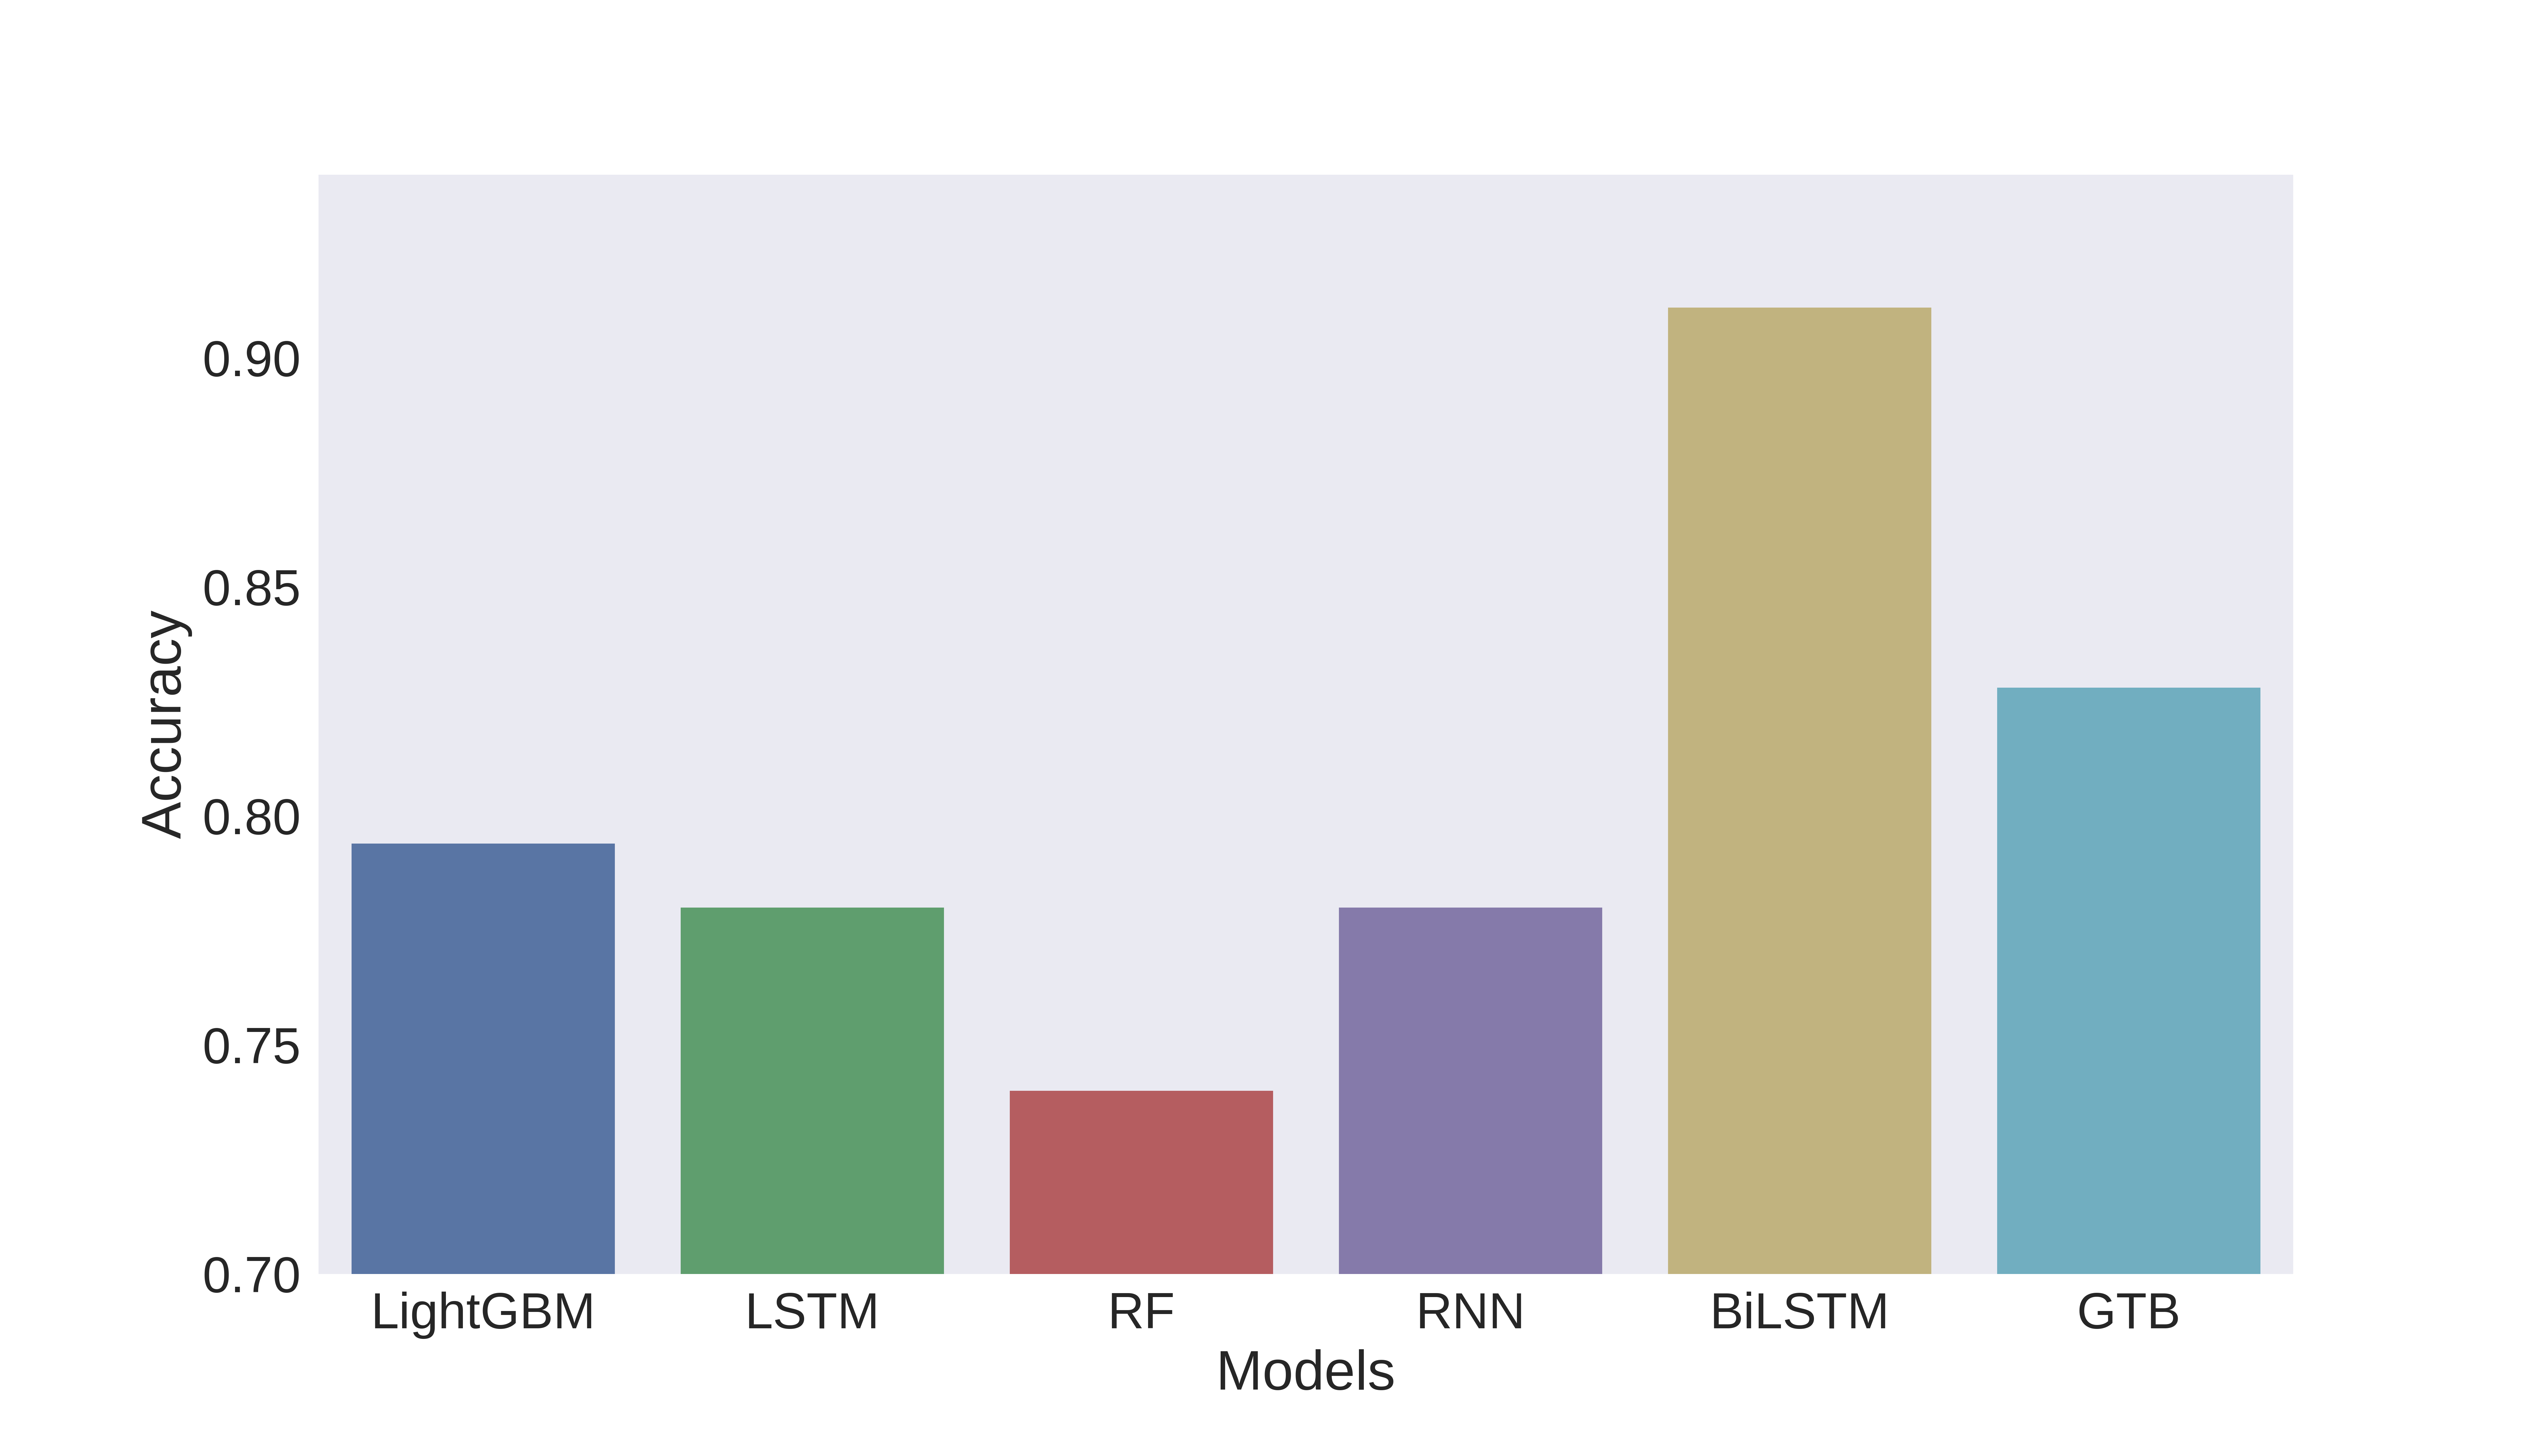
\includegraphics[scale=0.7,width=\linewidth]{UNSW_NB15_top_models_accuracy.png}
% \caption{Accuracy on UNSW-NB15}
% \end{figure}

% \begin{figure}
% \centering
%   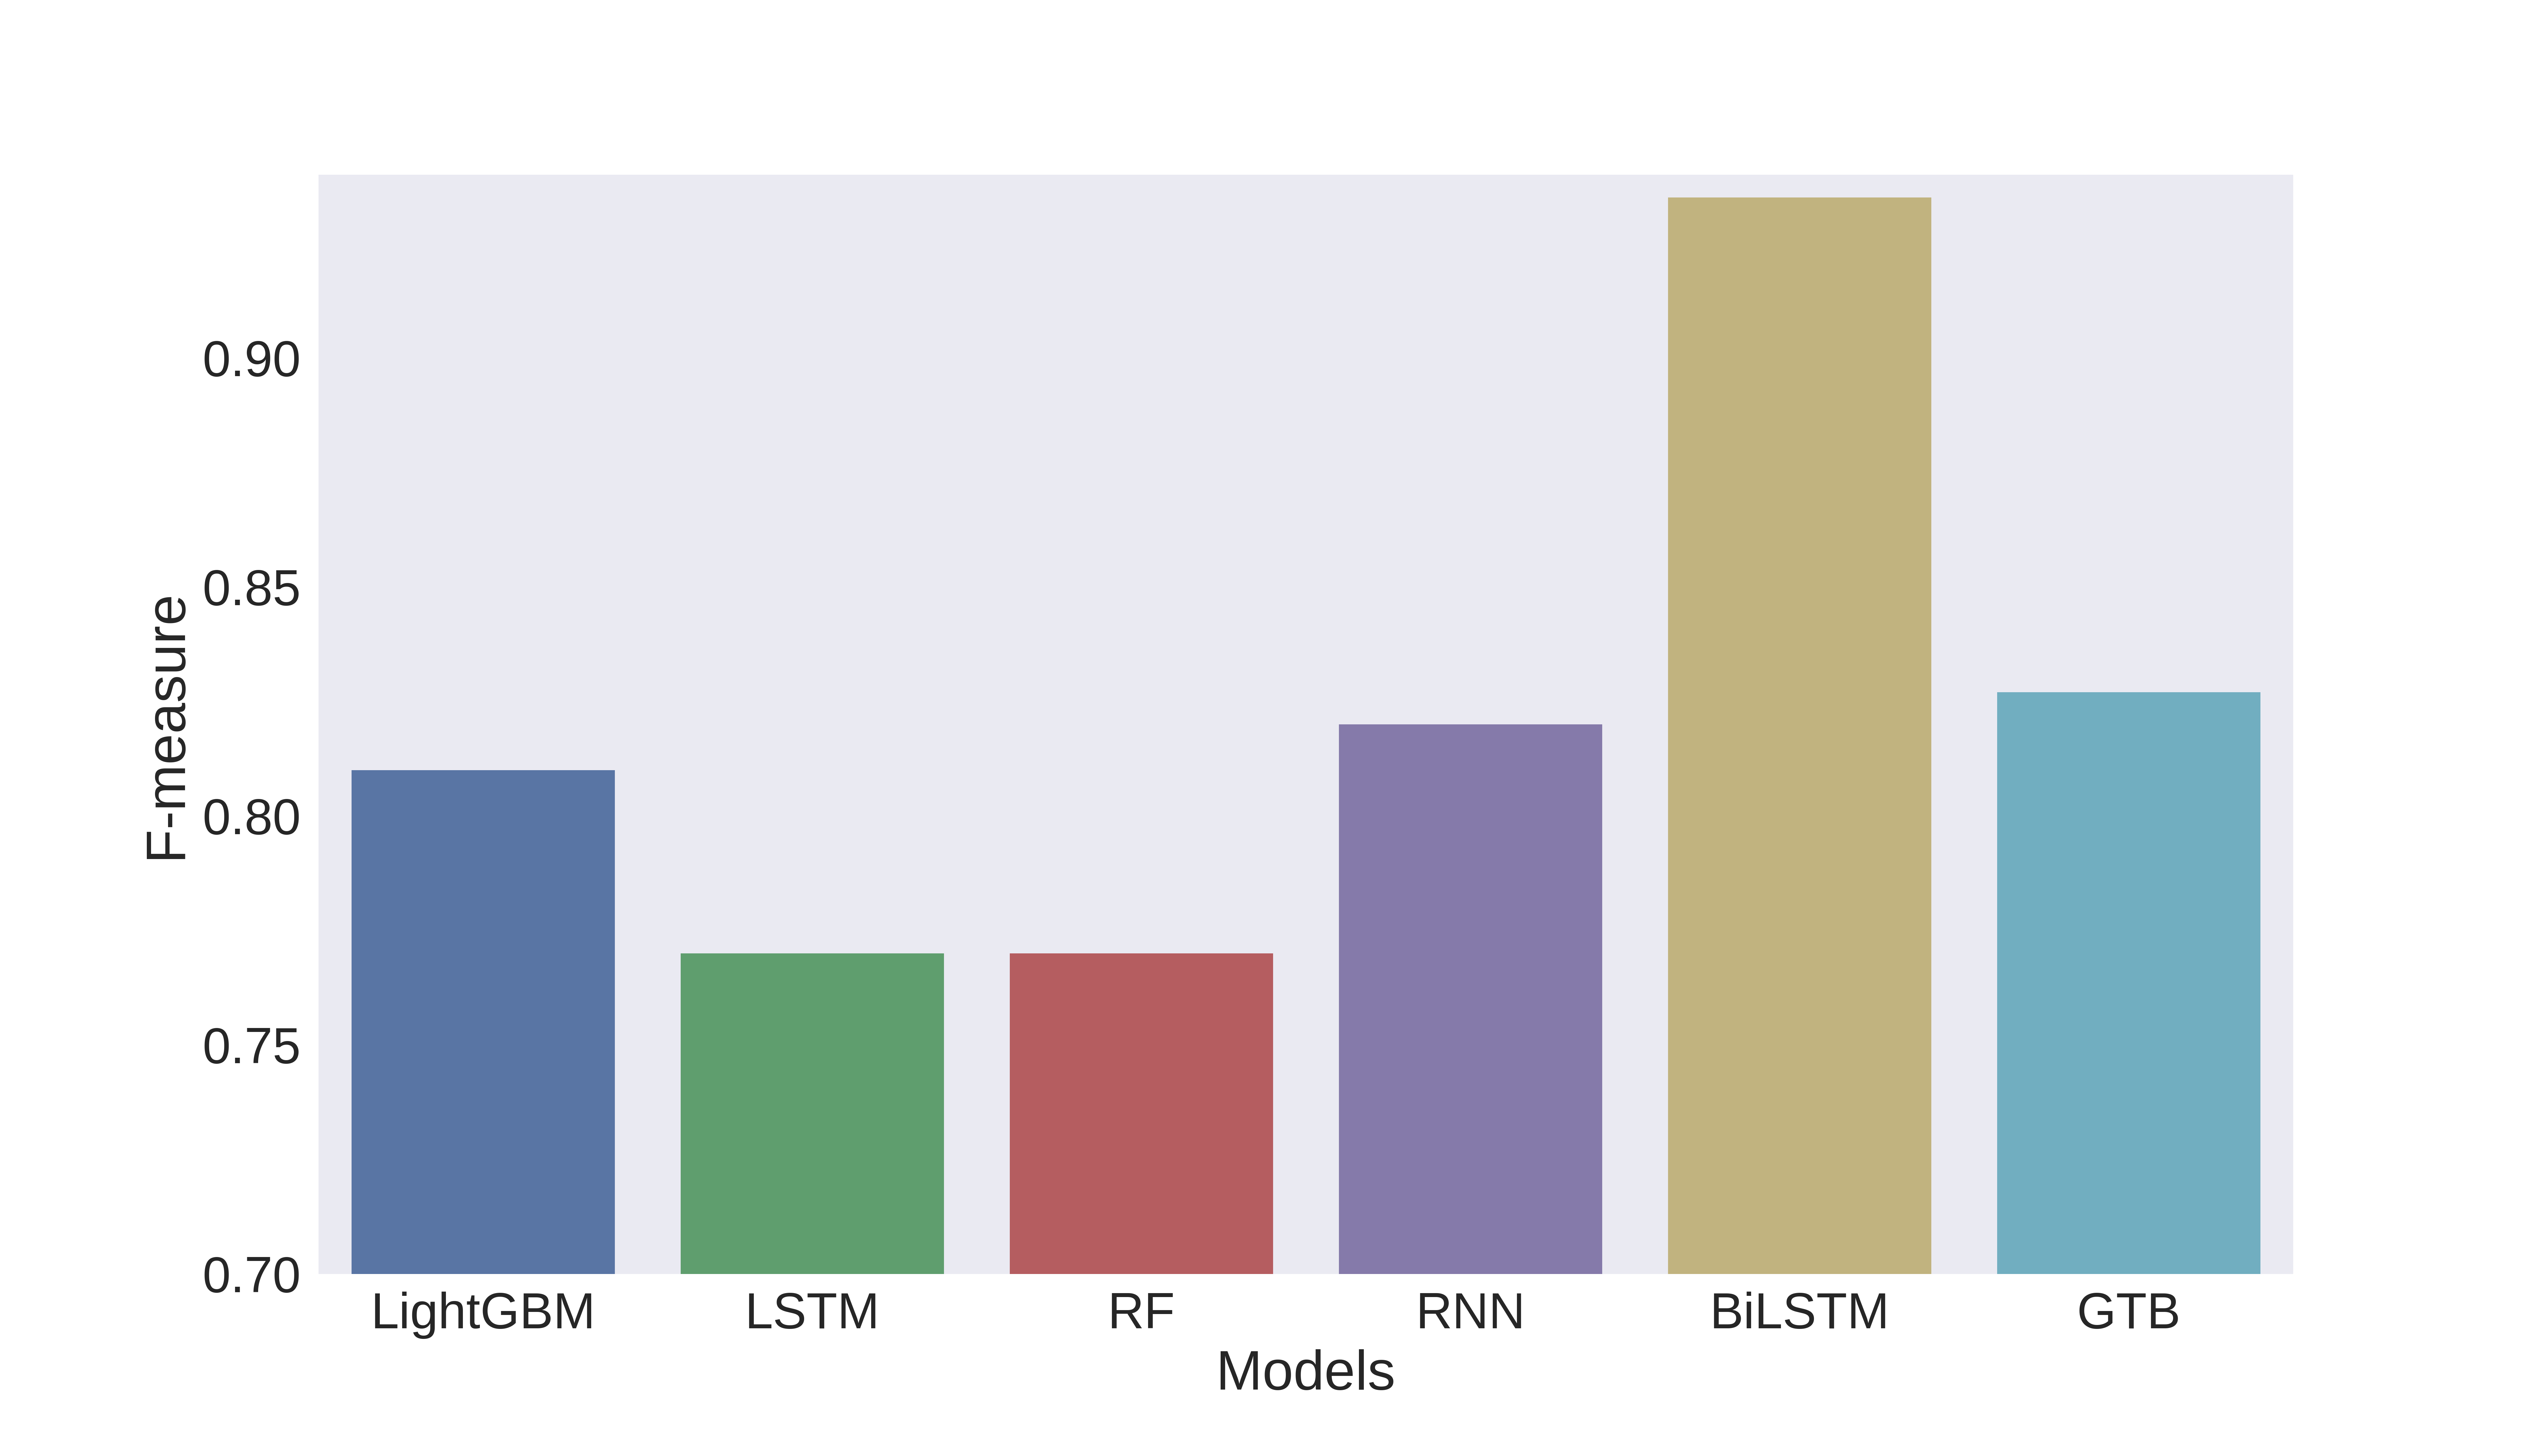
\includegraphics[scale=0.7,width=\linewidth]{UNSW_NB15_top_models_f_measure.png}

% \caption{F-measure on UNSW-NB15}
% \end{figure}

%---------------------------- Conclusion ----------------
%---------------------------- Conclusion ----------------
%---------------------------- Conclusion ----------------

\section{Conclusion and Future Work}
In this paper we have introduced an ensemble based machine learning model based on unsw-nb15. Our model outperforms in terms of detection rate and accuracy. However our limitations are model complexity and higher false positive rate.Yet its an indication of success of this kind of technique to go beyond previous state of the art works, which is promising. \\
In future we plan to investigate how ensemble can improve other anomaly detection works. We also want to explore the results of this technique on multi-class classification on this dataset and others. As some attacks are rarer than others, they are more difficult to detect than other common attacks. So these fields can also be explored, to effectively detect attacks which are harder to recognize.



\bibliography{bibliography} 

\end{document}


